%----------------------------------------------------------------------------
\chapter{Irodalomkutatás és a felhasznált technológiák}
\label{ch:tech}
%----------------------------------------------------------------------------
\section{A felhasznált technológiák ismertetése}
%----------------------------------------------------------------------------
Mivel a feladat egy specifikus alkalmazás előállítása volt, amely már létező termékek közötti kommunikációt biztosít, ezért ennek jelentős része volt a termékekkel való alapszintű, valamint a felhasznált specifikus funkciókkal és interfészekkel való mélyebb ismerkedés.


\subsection{IBM Security QRadar SIEM}
\label{subsec:qradar}
Az IBM Security QRadar SIEM az IBM security information and event manager rendszere, ami lehetővé teszi hálózatra csatlakoztatott eszközöknek a megfigyelését biztonsági szempontból. A hálózaton elosztott több ezernyi eszközvégpontból és alkalmazásból származó napló fájl eseményadatait összesíti, és a nyers adatokon azonnali normalizálási és összesítési műveleteket végez. Az eseménynaplók betöltésére számos automatikus módszer áll rendelkezésre, többek közt olyan közismert protokollok mint a SYSLOG, SNMP, FTP, SCP. Az IBM Security QRadar SIEM ugyancsak képes a rendszer sebezhetőségeinek és az esemény- és hálózati adatoknak az összevetésére, ezáltal segítséget nyújt a biztonsági incidensek rangsorolásában. Emellett lehetőség van egyéb adatforrások felvételére a felhasználó által is, amelyek szintén használhatók a fenyegetések és az incidensek detektálásában. Ezek jelentősége elsősorban a dinamikus szabályok létrehozásában játszik nagy szerepet, mivel ezek segítségével egy API-n keresztül karbantarthatók a létrehozott dinamikus szabályok. A szinkronizáció megvalósítására nincs egységes módszer vagy eszköz, ezt minden esetben az adatok jellege és az adatforrás által biztosított interfész határozza meg.

\begin{figure}
	\centering
	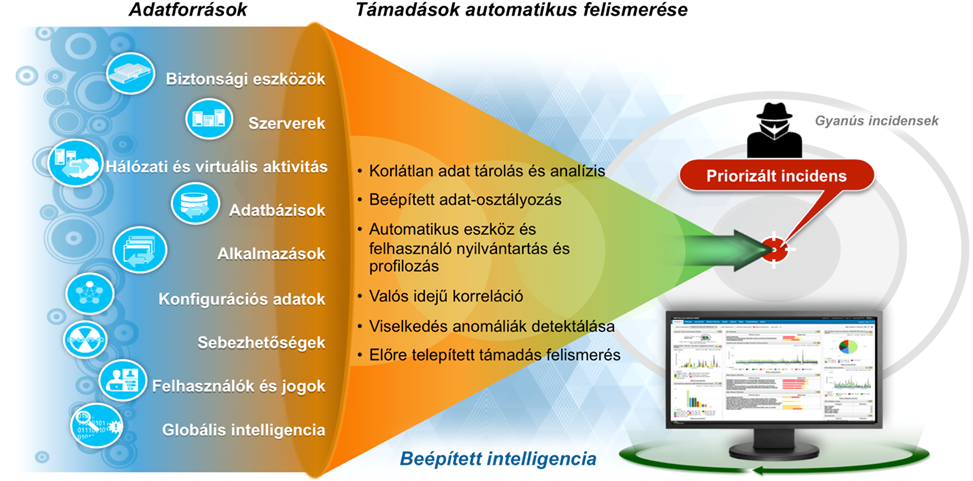
\includegraphics[width=0.9\linewidth]{figures/QRadar_promo.png}
	\caption{QRadar funkciói.}
	\label{fig:qradar-promo}
\end{figure}

Felvehetők a SIEM-be bizonyos sablonok alapján összeállítható szabályok, amelyeket a rule engine kiértékel a beérkező eseményekre. A kiértékelés alapján az eseményeket besorolja a megfelelő csoportokba súlyosságuk és egyéb tulajdonságaik alapján, vagy ha szükséges létrehoz egy új, különálló eseményt. Az incidensek kezelésére külön felület szolgál, illetve különböző interfészeken keresztül értesítést tud küldeni ezekről a rendszer. Ezen túl minden feldolgozott esemény később megtekinthető keresések és szűrések segítségével.

A SIEM által kiértékelt eseményekhez egyéb információkat is rendel a rendszer, olyanokat, mint például a támadás típusa, az esemény leírása, a résztvevő felek adatai, melyeket később is meg lehet tekinteni, valamint segítségükkel és az egyéb környezeti forgalommal együtt egy egész hálózat működése visszajátszható.
%\begin{comment}
%	A plusz információk közé tartozik egy 3 szempontú értékelés is, amely alapján a QRadar számolja az egyes esetek súlyosságát.
%	\begin{itemize}
%	\item Súlyosság (Severity) - a súlyosság jelzi hogy a támadó milyen fenyegetettséget jelent annak függvényében hogy mennyire sebezhető a megcélzott eszköz.
	
%	\item Hitelesség (Credibility) – a hitelesség jelzi az integritását vagy valódiságát egy támadásnak, amelyik érték az eseményt generáló biztonsági eszköztől érkezik. A hitelesség növekedhet, ha a különböző források is jelentik ugyanazt az eseményt.
	
%	\item Relevancia (Relevance) – a relevancia meghatározza azt, hogy a célpont milyen értéket képvisel a hálózaton.
%	\end{itemize}
%\end{comment}
 
\label{lbl:reference_data}
Ezen dokumentum és a feladat szempontjából a legfontosabb része a QRadarnak a dinamikusan feltölthető adathalmazok és azok használata szabályokban. Ezekkel a szabályokkal érhető el, hogy más adatforrásokból (jelen esetben az ISIM-ből) frissen feltöltött információk alapján változzon a kiértékelés, és ha valamilyen adat frissül, akkor naprakész maradjon a szabály által talált incidensek halmaza. A dinamikusan feltölthető adathalmazok (összefoglaló nevükön reference data) elérhetők egy REST API-n keresztül, így könnyen hozzájuk lehet férni és módosítani őket. Négy féle ilyen adathalmaz áll rendelkezésre:

\begin{itemize}
	\item Reference set - Olyan adathalmaz, melyben egyedi értékek sorozata található.
	\item Reference map - Olyan adathalmaz, melyben kulcs-érték párok találhatók, a kulcsok egyediek, és szigorúan szöveges adatok.
	\item Reference map of sets - Olyan adathalmaz, melyben kulcs-halmaz párok találhatók, a kulcsok egyediek, szövegesek, és a halmazban saját csoportjukban egyedi értékek találhatók.
	\item Reference map of maps (tables) - Olyan adathalmaz, melyben kulcs-kulcs-érték triplet összerendelések találhatók.
\end{itemize}

Minden reference data-nak van egy típusa, ami meghatározza hogy az adott halmazban milyen típusú értékek találhatók.

\begin{itemize}
	\item ALN - Alfanumerikus karakterek
	\item ALNIC - Alfanumerikus karakterek, figyelmen kívül hagyva a kis- és nagybetű közti különbséget 
	\item IP - IP címek
	\item NUM - Numerikus karakterek
	\item PORT - Port számok
	\item DATE - Dátumok, miliszekundomokban 1970.01.01 óta
\end{itemize}

Emellett a reference data-ban található adatoknak lehet egy TTL értéke is, ami meghatározza, hogy mennyi idő elteltével törlendő az adott adat. Ennek 3 típusa lehet: 
\begin{itemize}
	\item UNKNOWN - \todo
	\item LAST\_SEEN - Az adat utolsó feltöltésétől számítva kalkulálódik a TTL
	\item FIRST\_SEEN - Az adat első feltöltésétől számítva kalkulálódik a TTL
\end{itemize}

A feladat megvalósítása során az ISIM-ből kinyert adatokat ilyen reference data-kba töltjük fel, a típust úgy változtatva, ahogy az indokolt a kinyert adat szempontjából. A dolgozat nem foglalkozik a már feltöltött adatok további felhasználásával valamint a dinamikus szabályrendszer használatával, pusztán az integráció megvalósítására koncentrál.

\subsection{IBM Security Identity Manager - ISIM}
\label{subsec:ISIM}
Az IBM Security Identity Manager alapú IDM megoldás elsődleges feladata érzékelni a személyügyi változásokat, és egy központi szabálymotor alapján gondoskodni arról, hogy az alkalmazottak azokkal és csak azokkal a jogosultságokkal rendelkezzenek, amelyek mindenkori munkakörük beteljesítéséhez szükségesek.

Az ISIM tartja karban a kapcsolatot a vállalatnak dolgozó személyek és e személyek IT hozzáférései, jogosultságai között, gondoskodva mind a személyekben, mind a fiókokban bekövetkezett változások az aktuális biztonsági házirend alapján történő szinkronizálásáról. Ennek megfelelően két fő folyamatot definiál a rendszer.
Egyrészt a HR forrásokban, tehát a személyek adataiban bekövetkező változások hatásait kell érvénybe léptetni. Másrészt szükséges a menedzselt rendszeren (service) bekövetkezett, IDM-en kívül eszközölt módosítások detektálása, és azok átvezetése vagy korrigálása a belső szabályrendszernek megfelelően. 

Az ISIM ezen információk tárolására két külső adattárolót használ: egy LDAP alapú címtárban tárolja a modell entitásokat, azaz a személyek és fiókok adatait, rendszeradatokat, munkafolyamat és házirend definíciókat. Emellett használ egy relációs adatbázist a tranzakciós adatok, azaz a workflow példányok futási kontextusa (például aktív jog igénylések), audit bejegyzések, ideiglenes szimulációs és ütemezési adatok tárolására. Az integrációs modul használata folyamán ebből a két adattárolóból nyerjük ki az adott use-case-hez szükséges információkat.

\begin{figure}
	\centering
	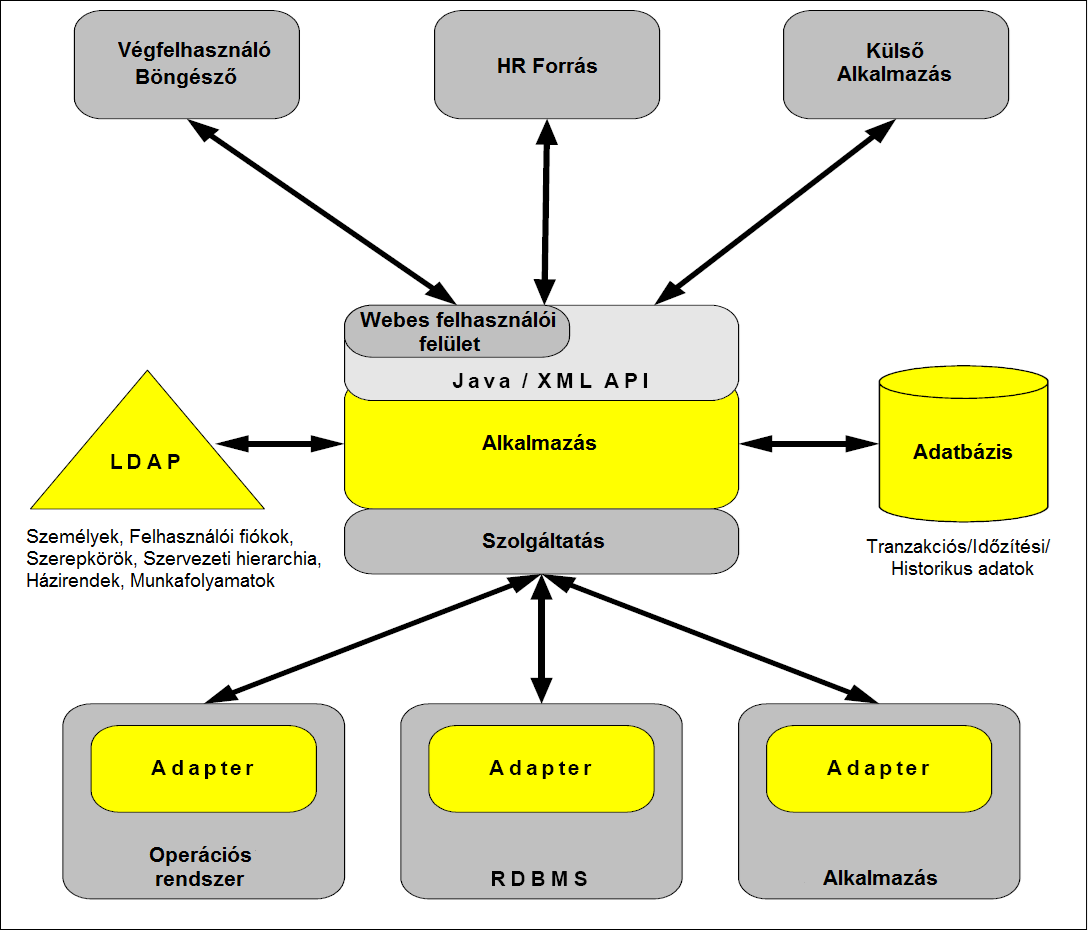
\includegraphics[width=0.5\linewidth]{figures/ISIM_promo.png}
	\caption{Az ISIM architektúrája és interfészei.}
	\label{fig:isim-promo}
\end{figure}


\subsection{Tivoli Directory Integrator - TDI}
\label{subsec:TDI}
A Tivoli Directory Integrator egy általános célú integrációs eszköz, ami lehetővé teszi több, különböző adatforrás koordinálását és integrációját. Mivel a legtöbb forrás más formátumot használ, és máshogy tárolja az adatot, egy ilyen integrációs lépés során szükséges bizonyos átalakításokat elvégezni az adatokon, valamint lehetséges hogy egyéb, plusz lépéseket is szükséges bevezetni, akár más adatforrások bevonásával. Ennek a procedúrának ad keretet a TDI egy grafikus fejlesztő felülettel, valamint a megfelelő Java alapú interfészekkel és kötésekkel, amelyek könnyűvé teszik új komponensek fejlesztését.

A TDI alapvető struktúrája úgynevezett assembly line-okból áll. Egy assembly line jelképez egy adat transzfert, a kezdeti adatok felolvasásától az átalakításokon át, a végső kimenet feltöltéséig. A ki- és bemeneti interakció ún. connectorokon keresztül történik, amelyek egy egységes interfészt implementálnak, és valamilyen külső adatforráshoz való kapcsolódást valósítanak meg. Minden connector, attól függően, hogy milyen műveletet végez 8 mód egyikében működik\footnote{A módok pontos leírása megtalálható a \ref{subsec:connimpl} szekcióban.}, valamint vagy aktív, vagy passzív módon dolgozik. Az előbbinél része az assembly line soros végrehajtásának, másikban nem, de külső vezérléssel működtethető.

A legtöbb adatforrás eltérő formátumban kezeli az adatokat, így TDI minden be- valamint kimeneti műveletnél biztosít egy hozzárendelési lépést, amellyel megadhatjuk, hogy a külső attribútumok milyen belső attribútumokra legyenek leképezve. Ilyen ún. mapping lépést az assembly line-on bármikor végrehajthatunk, és emellett még számos átalakítási lépés áll rendelkezésre, mint például ciklusok vagy elágazások használata. Az assembly line-on haladó adatokat entry-k\footnote{\href{https://www.ibm.com/support/knowledgecenter/en/SSCQGF_7.1.0/com.ibm.IBMDI.doc_7.1/entryobject.htm}{A TDI Entry osztály leírása a hivatalos IBM dokumentációban.}} formájában kezeli a TDI. Egy entry egy elemi objektum, ami nevesített attribútumok halmazát képes tárolni. Ilyen entry-t bármelyik scriptben létre lehet hozni, de egy általános TDI assembly line esetén 4 darab nevesített entry-t használunk:

\begin{itemize}
	\item work: Az assembly line állandó entry-je. Ezen az objektumon keresztül utazik az adat az egyes komponensek között, valamint ezen hajtják végre az adatmódosító műveletket a connector-ok.
	\item conn: Ezt az entry objektumot használják a connecot-ok a köztes adatok tárolására a célrendszerrel való kapcsolat során. Ebből az entry-ből kerülnek át az egyes mapping-ek során az adatok a work entry-be.
	\item current: Bizonyos connector-ok update módjainál elérhető változó, ami a csatlakoztatott rendszeren található adatokat tartalmazza.
	\item error: A hibakezelést végző komponensekben elérhető entry. A hibákkal kapcsolatos információkat tartalmazza.
\end{itemize}

A TDI talán egyik legfontosabb képessége a Javascriptből való testreszabhatóság. Ez azt jelenti, hogy az assembly line-on az adatokat szabadon manipulálhatjuk Javascriptes kódból, létrehozhatunk szkripteket amik a futtatás bizonyos pontjain aktiválódnak, valamint számtalan egyéb funkciót érhetünk el ezekből a programokból, mint például a logolás, paraméterek módosítása, vagy arbitrális kód futtatása.

A dolgozat szempontjából az egyik legfontosabb része a TDI-nak a connectorok, mivel a feladat része volt egy ilyen fejelsztése, ami támogatja a kommunikációt egy QRadar szerverrel, azon belül is a QRadarban található reference data objektumokkal.
